\chapter{Исследовательская часть}

\section{Технические характеристики}

Ниже приведены технические характеристики устройства, на котором выполнялось тестирование.

\begin{itemize}
	\item Операционная система: macOS 14.6.1.
	\item Объём оперативной памяти: 18 Гб.
	\item Процессор: Apple M3 Pro.
\end{itemize}

Тестирование проводилось на ноутбуке, включённом в сеть электропитания. Во время тестирования ноутбук был нагружен только встроенными приложениями окружения, а также непосредственно системой тестирования.

% 

\section{Время выполнения реализаций алгоритмов}

Алгоритмы тестировались при помощи функции process\_time() из библиотеки time языка Python. Данная функция всегда возвращает значения времени в секундах типа float, которые являются суммой системного и пользовательского процессорного времени процессора, на котором выполнялась программа.~\cite{pythonlangtime}

Среднее время выполнения генетического алгоритма составило 149.64 с. для аппроксимации функции $f(x)$ и 117.12 с. для $g(x)$. Результат аппроксимации функции $f(x)$: 
\begin{equation}
	\phi_f(x, \overline{a}) = -0.045774x^5-0.032708x^4+1.996497x^3+1.078365x^2-16.730258x-3.44288,
\end{equation}
\begin{equation}
	\sigma_f = 17.544.
\end{equation}

Результат аппроксимации функции $g(x)$: 
\begin{equation}
	\phi_g(x, \overline{a}) = 0.99128784x^3 + 0.00712201x^2 -0.88137867x + 2.93948756,
	\end{equation}
	\begin{equation}
	\sigma_g = 0.177.
\end{equation}

На рисунках \ref{img:fitness_f} и \ref{img:fitness_g} приведены графики зависимостей между числом пройденных поколений оптимизации и похожестью между аппроксимирующей и аппроксимируемой функциями.

\begin{figure}
	\begin{center}
		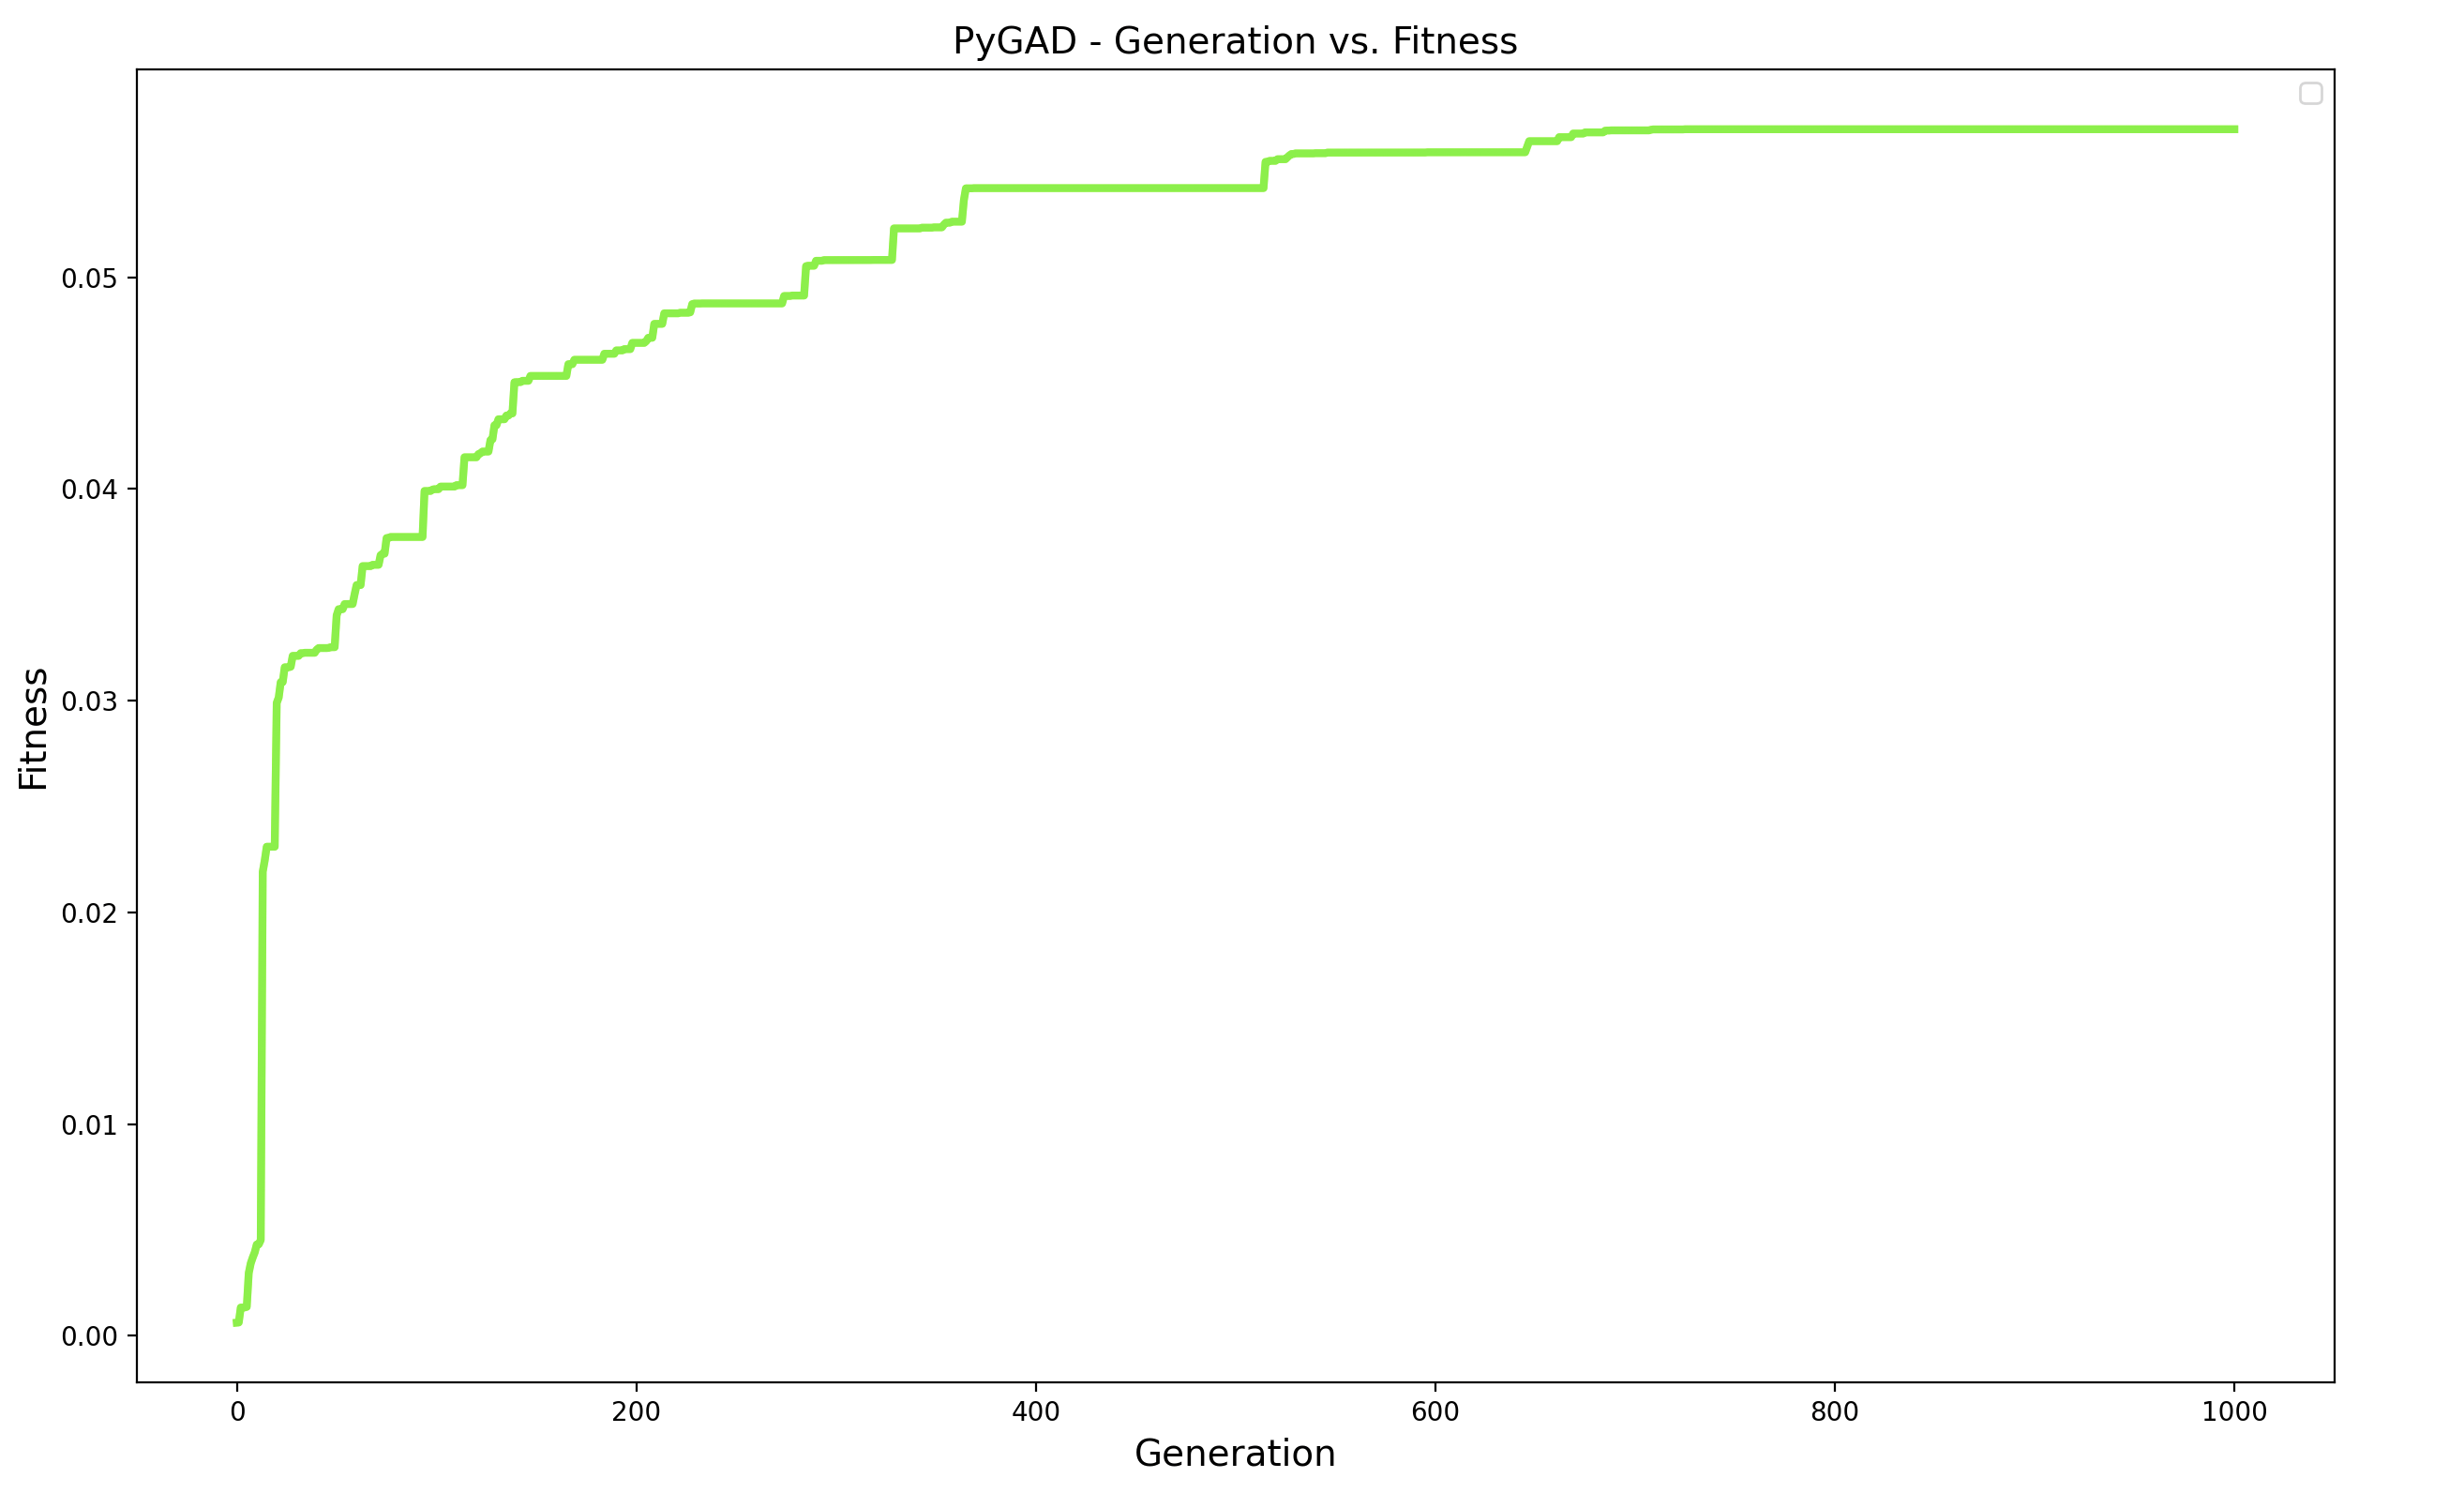
\includegraphics[width=0.9\textwidth]{images/1.png}
	\end{center}
	\caption{Зависимость похожести $f(x)$ и $\phi_f(x, \overline{a})$ от числа пройденных поколений оптимизации}
	\label{img:fitness_f}
\end{figure}

\begin{figure}
	\begin{center}
		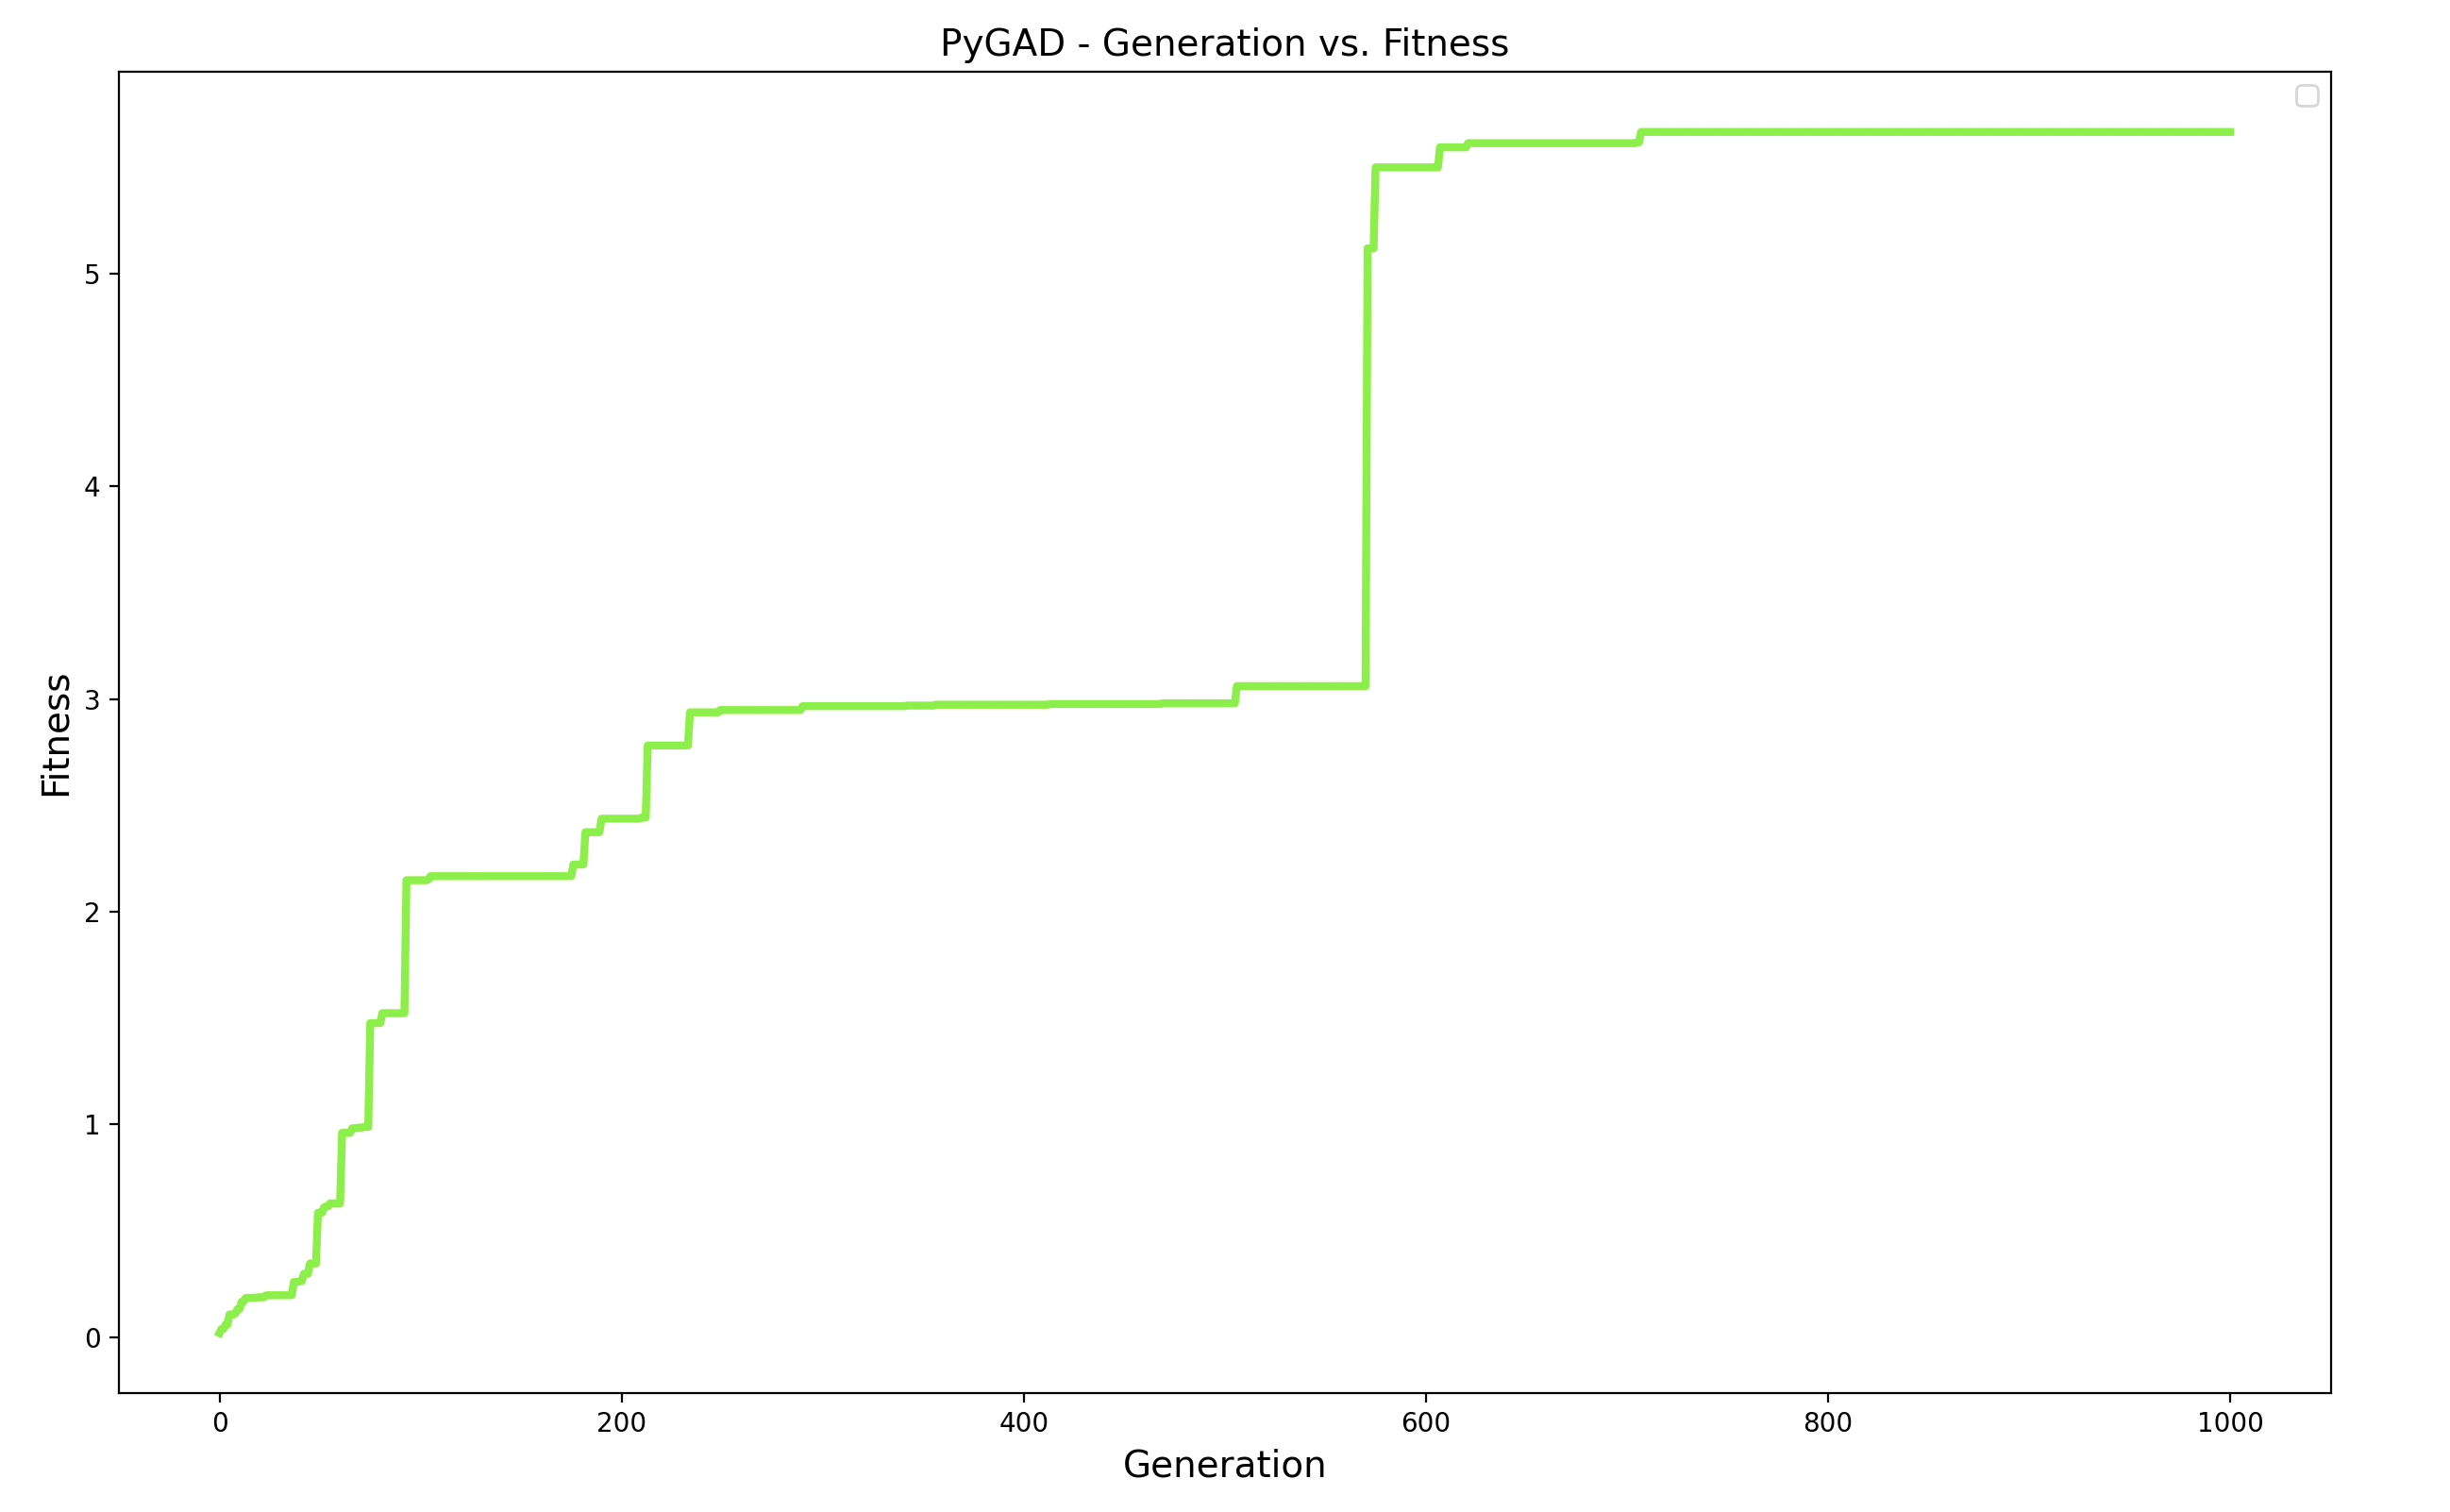
\includegraphics[width=0.9\textwidth]{images/2.png}
	\end{center}
	\caption{Зависимость похожести $g(x)$ и $\phi_g(x, \overline{a})$ от числа пройденных поколений оптимизации}
	\label{img:fitness_g}
\end{figure}

Среднее время выполнения эволюционного алгоритма составило 173.17 с. для аппроксимации функции $f(x)$ и 128.098286 с. для $g(x)$. Результат аппроксимации функции $f(x)$: 
\begin{equation}
	\phi_f(x, \overline{a}) = -17.00417829x^5-3.73938996x^4-17.54370723x^3+20x^2-1.720966x+20,
	\end{equation}
	\begin{equation}
	\sigma_f = 25.447.
\end{equation}

Результат аппроксимации функции $g(x)$: 
\begin{equation}
	\phi_g(x, \overline{a}) = 0.48981863x^3+0.21815401x^2+0.14574346x+0.00134332,
	\end{equation}
	\begin{equation}
	\sigma_g = 8.591.
\end{equation}

\section*{Вывод}

В данном разделе были приведены результаты замеров времени выполнения алгоритмов аппроксимации функций. При сравнимом времени выполнения эволюционный алгоритм на основе муравьиной кучи показал меньшую точность, чем генетический алгоритм: для $f(x)$ среднеквадратичная ошибка была в 1.5 раз больше, для $g(x)$ --- в 48 раз больше.

\clearpage
